\documentclass{article}
\usepackage{tikz}
\usetikzlibrary{decorations.text}

\begin{document}

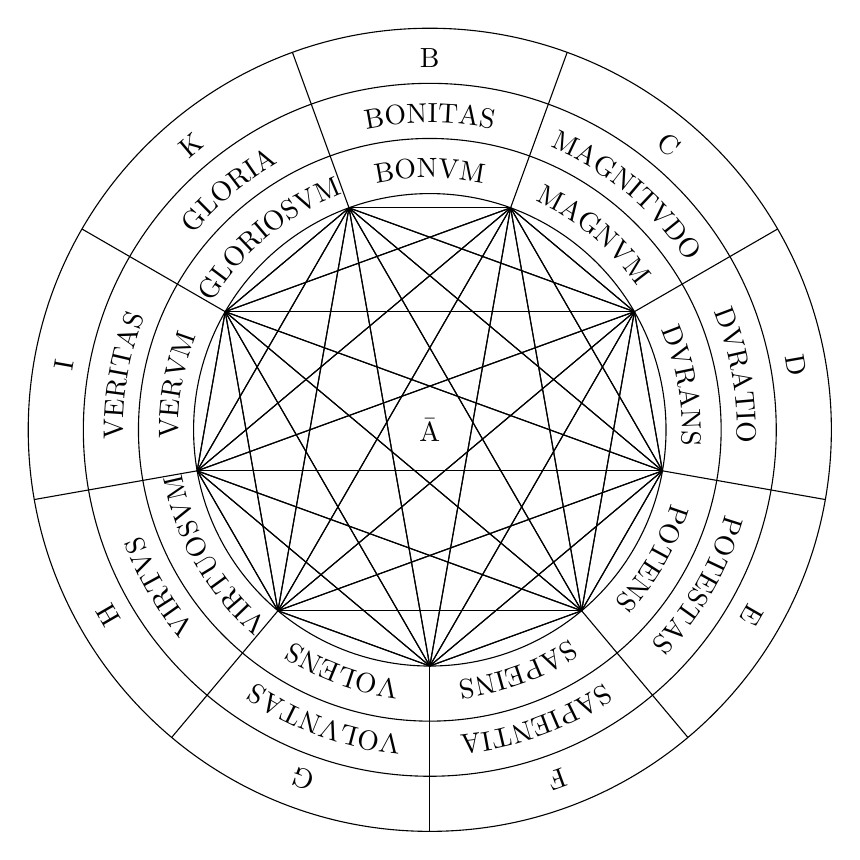
\begin{tikzpicture}

\draw (0,0) node {Ā}; % Central Alpha

% Rings
\foreach \r in {3,3.7,4.4,5.1}
  \draw (0,0) circle [radius=\r cm];

% Rays
\foreach \x in {0,...,8}
  \draw (270+40*\x:3cm) -- (270+40*\x:5.1cm);

% Rings of Text
\foreach \y in {0,1,2} %
  \foreach \x in {0,...,8} {

    \pgfmathparse{{{"VOLENS","VIRTUOSVM","VERVM","GLORIOSVM","BONVM","MAGNVM","DVRANS","POTENS","SAPEINS"},
                   {"VOLVNTAS","VIRTVS","VERITAS","GLORIA","BONITAS","MAGNITVDO","DVRATIO","POTESTAS","SAPIENTIA"},
                   {"G","H","I","K","B","C","D","E","F"}}[\y][\x]}
    \edef\letter{\pgfmathresult}

    \draw [decoration={
            text along path,
            text={\letter},
            text align={center}
           },
           decorate]

      (270-40*\x:3.2cm+0.7cm*\y) % Start Location

      arc[start angle=270-40*\x,
          delta angle=-40,
          radius=3.2cm+0.7cm*\y];
}

% Connecting Lines

\foreach \y in {0,...,8} {
  \pgfmathtruncatemacro{\maxx}{8-\y} % Classic TikZ Gotcha
  \foreach \x in {0,...,8} {
    \draw (270+40*\y:3cm) -- (270+40*\x:3cm);
  }
}

\end{tikzpicture}

\end{document}
usepackage{tikz}
\usetikzlibrary{decorations.text}

\begin{document}

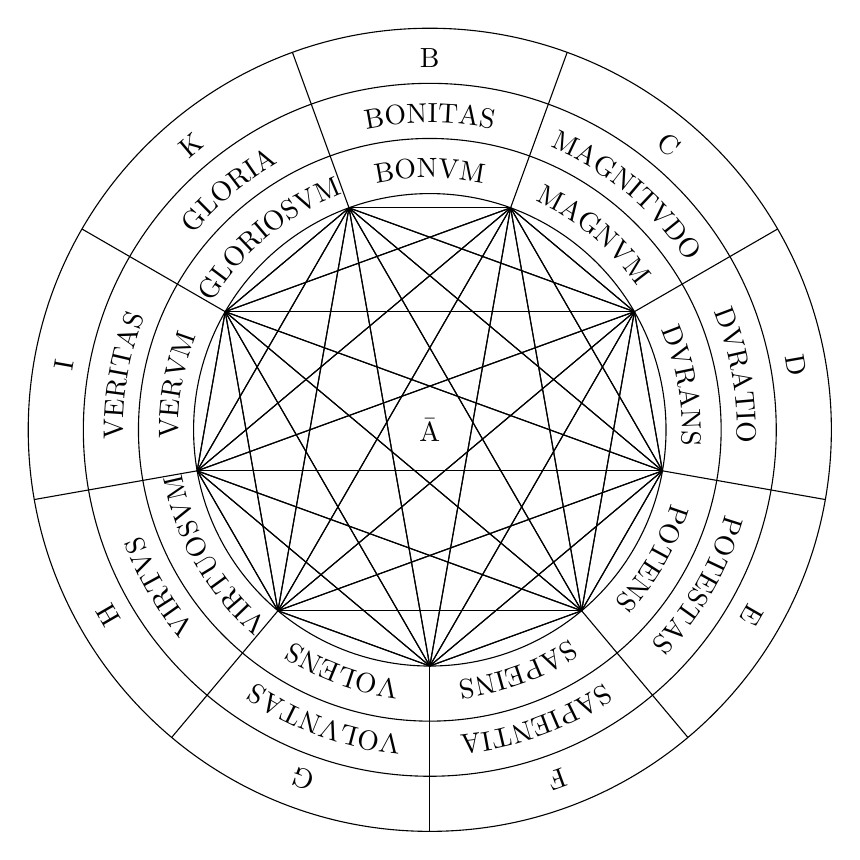
\begin{tikzpicture}

\draw (0,0) node {Ā}; % Central Alpha

% Rings
\foreach \r in {3,3.7,4.4,5.1}
  \draw (0,0) circle [radius=\r cm];

% Rays
\foreach \x in {0,...,8}
  \draw (270+40*\x:3cm) -- (270+40*\x:5.1cm);

% Rings of Text
\foreach \y in {0,1,2} %
  \foreach \x in {0,...,8} {

    \pgfmathparse{{{"VOLENS","VIRTUOSVM","VERVM","GLORIOSVM","BONVM","MAGNVM","DVRANS","POTENS","SAPEINS"},
                   {"VOLVNTAS","VIRTVS","VERITAS","GLORIA","BONITAS","MAGNITVDO","DVRATIO","POTESTAS","SAPIENTIA"},
                   {"G","H","I","K","B","C","D","E","F"}}[\y][\x]}
    \edef\letter{\pgfmathresult}

    \draw [decoration={
            text along path,
            text={\letter},
            text align={center}
           },
           decorate]

      (270-40*\x:3.2cm+0.7cm*\y) % Start Location

      arc[start angle=270-40*\x,
          delta angle=-40,
          radius=3.2cm+0.7cm*\y];
}

% Connecting Lines

\foreach \y in {0,...,8} {
  \pgfmathtruncatemacro{\maxx}{8-\y} % Classic TikZ Gotcha
  \foreach \x in {0,...,8} {
    \draw (270+40*\y:3cm) -- (270+40*\x:3cm);
  }
}

\end{tikzpicture}

\end{document}
